% =============================================================================
%  MIRROR - IEEE workshop variant #2
%  Target venue: The 6th International Workshop on Multi-Modal Medical Data
%                Analysis (a workshop of IEEE BigData)
%
%  This file is a reframing of the SSRN/arXiv preprint (paper/main.tex, v10) into
%  IEEEtran conference format. NO measured number is changed: every figure, table,
%  and result is copied from main.tex, which in turn traces to committed JSON under
%  results/ and to paper/calibration_baseline.py. Only the framing (title,
%  abstract, introduction, the dedicated Section on multi-modal analysis, the
%  discussion emphasis, and the conclusion) is customized to this workshop's theme.
%  The honest scope is preserved unchanged: three modalities are registered,
%  routed, and tested; only chest X-ray is trained and benchmarked.
%
%  Engine: pdfLaTeX, no bibtex step (bibliography embedded). The three UI
%  screenshots live in ../figures/ and are guarded by \IfFileExists, so the file
%  still compiles if they are absent. Two passes resolve cross-references.
% =============================================================================
\documentclass[conference]{IEEEtran}
\IEEEoverridecommandlockouts

\usepackage{cite}
\usepackage{amsmath,amssymb}
\usepackage[T1]{fontenc}
\usepackage{graphicx}
\usepackage{booktabs}
\usepackage{array}
\usepackage{enumitem}
\usepackage{xcolor}
\usepackage{tikz}
\usepackage{pgfplots}
\pgfplotsset{compat=1.18}
\usetikzlibrary{arrows.meta,positioning}
\usepackage[hidelinks]{hyperref}
\usepackage{url}

% Do not strand a single line of a paragraph at a column boundary.
\widowpenalty=10000
\clubpenalty=10000
\displaywidowpenalty=10000

\definecolor{mirrorblue}{RGB}{31,86,145}
\definecolor{mirrorgray}{RGB}{90,96,104}
\definecolor{boxbg}{RGB}{237,243,250}

\newcommand{\code}[1]{\texttt{\small #1}}

% Run-in bold lead: a paragraph that opens in bold, nothing more. Every bold
% lead-in in the paper goes through this so they cannot drift apart. Precede each
% call with a blank line in the source to start a fresh paragraph.
\newcommand{\rih}[1]{\textbf{#1}\enspace\ignorespaces}

% Include the screenshot if present, else a labelled placeholder box.
% #1 = path, #2 = width, #3 = fallback caption text.
\newcommand{\figorbox}[3]{%
  \IfFileExists{#1}{\includegraphics[width=#2]{#1}}%
  {\fbox{\parbox[c][2.8cm][c]{#2}{\centering\color{gray}\itshape #3\\(add image to paper/figures/)}}}}

\hypersetup{pdftitle={MIRROR: One Pipeline, Three Modalities -- Registry-Driven Multi-Modal Grounded Radiology Reporting},
            pdfauthor={Vignesh Nagarajan}}

\begin{document}

\title{One Pipeline, Three Modalities: Registry-Driven\\
Multi-Modal Grounded Radiology Reporting in MIRROR}

\author{%
\IEEEauthorblockN{Vignesh Nagarajan}
\IEEEauthorblockA{\textit{Dept.\ of Computer Science \& Engineering}\\
\textit{Texas A\&M University}\\
College Station, TX, USA\\
vigneshn26@tamu.edu}
\and
\IEEEauthorblockN{Sriram Venkatapathy}
\IEEEauthorblockA{\textit{Applied AI Research}\\
\textit{Capital One}\\
PhD, IIT Hyderabad\\
sriram.venkatapathy@gmail.com}}

\maketitle

\begin{abstract}
Medical imaging is intrinsically multi-modal: a chest radiograph, a brain MRI, and
a head CT differ in their finding taxonomy, their anatomical vocabulary, and the
plane they are read in, and most pipelines hard-code one of them. MIRROR is a
research prototype whose per-modality differences, the label set, the vocabulary a
saliency centroid is named in, and a little report phrasing, live in one registry,
so the classification, localization, and reporting stages are modality-agnostic and
adding a modality is a data change rather than a code change. Three taxonomies are
registered and routed here, chest X-ray (14 NIH ChestX-ray14 labels), brain MRI (11
labels), and head CT (11 RSNA-derived labels), each dispatched explicitly or from a
study's DICOM modality tag, and the routing, head sizing, and anatomical vocabulary
are exercised by the test suite for all three. MIRROR also fuses modalities of
representation: it translates an image into structured evidence and then into text
through a language layer that receives the labels, probabilities, and regions but
never the pixels, so the report can assert only findings the classifier produced.
We are careful about scope. Only chest X-ray is trained and benchmarked; on the
ChestMNIST derivative the classifier reaches macro AUROC $0.729$ and ranks every
label $1.6$ to $6.8$ times better than chance, yet emits no positive prediction for
11 of 14 labels at the default threshold, a decision-versus-discrimination gap we
report against its no-skill floors. The brain-MRI and head-CT paths are
architectural: routed and tested, not yet trained.
\end{abstract}

\begin{IEEEkeywords}
multi-modal medical imaging, chest X-ray, brain MRI, head CT, DICOM, modality
registry, explainable AI, radiology report generation, grounding
\end{IEEEkeywords}

% -----------------------------------------------------------------------------
\section{Introduction}

Deep networks now match specialists on narrow chest-radiograph reading
tasks~\cite{rajpurkar2017chexnet}, yet adoption remains limited by a trust gap: a
bare probability tells a radiologist neither \emph{where} the model is looking nor
\emph{why} it concluded what it did, and high-stakes decisions demand models that
can be interrogated~\cite{rudin2019stop}. Saliency methods such as
Grad-CAM~\cite{selvaraju2017gradcam} expose \emph{where} a prediction comes from,
and language models can render structured evidence as prose, but the two are rarely
composed into one pipeline whose outputs stay mutually consistent, and whose trust
guarantees are stated precisely enough to be checked.

Composing them introduces a second risk the first does not have. A report
generator with access to the image can write fluent radiology prose asserting
findings no classifier ever produced, and such prose is difficult to audit
precisely because it reads well. MIRROR is built around a constraint aimed at that
risk: image $\rightarrow$ prediction $\rightarrow$ localization $\rightarrow$
reasoning $\rightarrow$ report, with the language layer receiving only the
structured evidence produced upstream, never the raw image. The report can
therefore assert only findings the classifier predicted and the localizer situated.

Most explainable-radiology work fixes one imaging modality and rebuilds the stack
for the next. MIRROR takes the opposite stance: only the finding taxonomy, the
anatomical vocabulary, and a little report phrasing differ between modalities, so
those three things are centralized in a single registry and the pipeline itself is
modality-agnostic. This paper reads MIRROR as a multi-modal medical-data analysis
system in two senses. Across imaging modalities, one registry-driven pipeline
routes and analyzes chest X-ray, brain MRI, and head CT, dispatching a study either
explicitly or from the modality tag in its DICOM header. Across modalities of
representation, the pipeline translates pixels into structured evidence and then
into a natural-language report, and it does so under a grounding constraint that
keeps the language modality faithful to the image modality it summarizes.

\rih{Research question.} Can one pipeline analyze several imaging modalities without
re-engineering the stack per modality, by treating each modality's taxonomy,
vocabulary, and phrasing as data; and can the image-to-text translation be
constrained so the language layer cannot assert a finding the classifier did not
detect? We answer both architecturally, and we measure the cost of the constraint
on the one modality we train, chest X-ray. Two things this paper does \emph{not}
answer should be stated at the outset. It reports no predictive result for brain MRI
or head CT, which are routed and tested but not trained. And it does not measure
explanation \emph{quality}: our harness implements a pointing-game and IoU protocol
against the NIH lesion boxes, but running it needs a checkpoint trained on the
full-resolution release, so no box-level score is reported here.

\rih{Contributions.}
\begin{enumerate}[leftmargin=1.3em,itemsep=1pt,topsep=2pt]
  \item A registry-driven multi-modality in which a modality's taxonomy, anatomical
  vocabulary, and report phrasing are data rather than code, so the classification,
  localization, and reporting stages are modality-agnostic. Three taxonomies are
  registered, routed, and exercised by the test suite; one is benchmarked.
  \item A grounded cross-modal translation from image to structured evidence to
  text, in which the language layer receives labels, probabilities, and regions but
  never the pixels, so the report can assert only findings the classifier produced,
  a property checkable by a unit test rather than a benchmark.
  \item A real DICOM ingest that applies the modality LUT, VOI LUT, and MONOCHROME1
  inversion, lifts only non-PHI tags, and exposes the modality tag for automatic
  routing, plus two very different inference engines behind one response contract.
  \item A measured chest-radiograph result in which discrimination is real on every
  label while decisions are absent on almost all of them, reported against the
  no-skill floors that make Brier and AUPRC interpretable under class imbalance.
\end{enumerate}

% -----------------------------------------------------------------------------
\section{Related Work}
\label{sec:litreview}

\rih{Datasets and classification.} Large labeled chest-radiograph corpora made
supervised deep learning on this modality practical. The NIH ChestX-ray8/14
release~\cite{wang2017chestxray} provides $112{,}120$ frontal radiographs over 14
pathologies; CheXpert~\cite{irvin2019chexpert} and MIMIC-CXR~\cite{johnson2019mimiccxr}
extended scale, uncertainty labeling, and paired reports. CheXNet~\cite{rajpurkar2017chexnet}
showed a 121-layer DenseNet~\cite{huang2017densenet} reaching radiologist-level
pneumonia detection. EfficientNet~\cite{tan2019efficientnet} and Vision
Transformers~\cite{dosovitskiy2021vit} complete the standard toolkit; MIRROR keeps
all three interchangeable, with DenseNet-121 primary for comparability.

\rih{Visual explanation.} Class Activation Mapping~\cite{zhou2016cam} localized the
evidence behind a CNN prediction; Grad-CAM~\cite{selvaraju2017gradcam} generalized
it to arbitrary architectures via gradients, and Score-CAM~\cite{wang2020scorecam}
removed the gradient dependence. Model-agnostic methods, notably
LIME~\cite{ribeiro2016lime} and SHAP~\cite{lundberg2017shap}, explain individual
predictions without model internals. The pointing-game protocol~\cite{zhang2016pointing}
and intersection-over-union against annotated lesions turn heatmaps into
quantitative localization scores; our harness implements both, though we do not run
them here.

\rih{Critiques of post-hoc explanation.} Adebayo et al.~\cite{adebayo2018sanity}
showed several saliency methods can be insensitive to the model and data they
purport to explain, and argued for sanity checks before any map is trusted.
Rudin~\cite{rudin2019stop} argued that high-stakes decisions call for inherently
interpretable models rather than post-hoc explanations, and Doshi-Velez and
Kim~\cite{doshivelez2017rigorous} called for a measurable science of
interpretability. MIRROR is the kind of system these critiques target, and we take
up its position against them in Section~\ref{sec:discussion} rather than citing
them only as background.

\rih{Report generation.} Systems emitting radiology prose range from
TieNet~\cite{wang2018tienet} to memory-driven transformers such as
R2Gen~\cite{chen2020r2gen} to decoders optimized for factual
correctness~\cite{liu2019clinically}. The recurring failure mode is hallucination:
prose generated directly from pixels can assert findings the model never detected.
Surveys of explainable AI in medical imaging~\cite{tjoa2021survey} note that
interpretability and report generation are usually studied separately. MIRROR's
contribution is neither a new classifier nor a new saliency method but their
composition under a constraint that bounds what the report may assert.

% -----------------------------------------------------------------------------
\section{System Architecture}
\label{sec:method}

MIRROR chains three layers; each layer's output is the grounded input to the next
(Fig.~\ref{fig:arch}).

\begin{figure}[tbp]
\centering
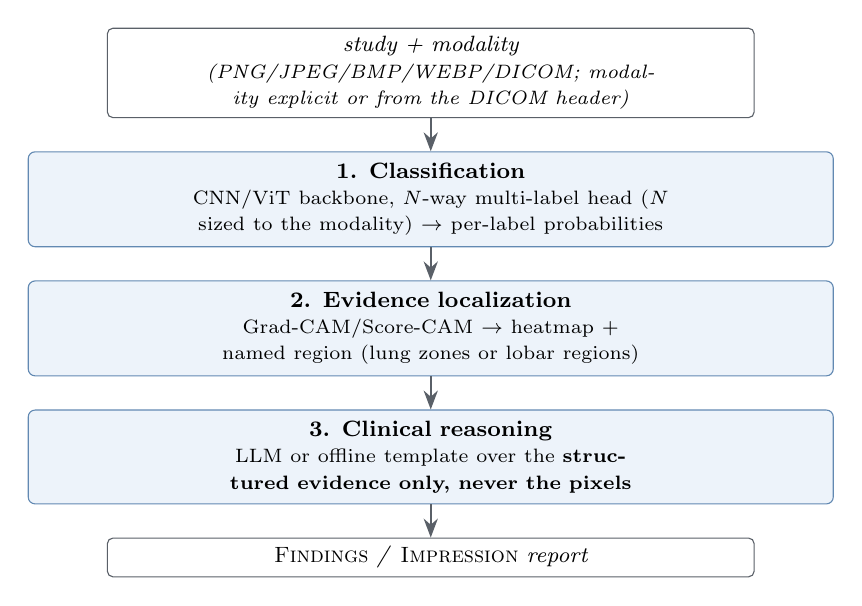
\begin{tikzpicture}[
  node distance=4.2mm,
  layer/.style={rectangle, rounded corners=2.5pt, draw=mirrorblue!70, fill=boxbg,
                text width=0.82\linewidth, align=center, inner sep=4pt,
                font=\footnotesize},
  io/.style={rectangle, rounded corners=2pt, draw=mirrorgray, fill=white,
             text width=0.66\linewidth, align=center, inner sep=3pt,
             font=\footnotesize\itshape},
  arr/.style={-{Stealth[length=2.4mm]}, thick, mirrorgray}
]
\node[io] (img) {study + modality \\ \scriptsize(PNG/JPEG/BMP/WEBP/DICOM;
   modality explicit or from the DICOM header)};
\node[layer, below=of img] (clf)
  {\textbf{1. Classification}\\ \scriptsize CNN/ViT backbone, $N$-way multi-label
   head ($N$ sized to the modality) $\rightarrow$ per-label probabilities};
\node[layer, below=of clf] (loc)
  {\textbf{2. Evidence localization}\\ \scriptsize Grad-CAM/Score-CAM
   $\rightarrow$ heatmap + named region (lung zones or lobar regions)};
\node[layer, below=of loc] (rep)
  {\textbf{3. Clinical reasoning}\\ \scriptsize LLM or offline template over the
   \textbf{structured evidence only, never the pixels}};
\node[io, below=of rep] (out) {\textsc{Findings} / \textsc{Impression} report};
\draw[arr] (img) -- (clf);
\draw[arr] (clf) -- (loc);
\draw[arr] (loc) -- (rep);
\draw[arr] (rep) -- (out);
\end{tikzpicture}
\caption{The MIRROR pipeline as deployed in the local PyTorch stack, the
configuration benchmarked in Section~\ref{sec:results}. Layers 2 and 3 are
individually toggleable, which recovers the conditions of
Section~\ref{sec:setup}. The hosted engine of Section~\ref{sec:serving} does not
have this structure.}
\label{fig:arch}
\end{figure}

\subsection{Layer 1: Classification}
The classifier is a factory over three ImageNet-pretrained backbones: DenseNet-121
(default), EfficientNet-B0, and ViT-B/16, with a multi-label head whose width $N$
is the size of the active modality's taxonomy (14 for chest X-ray, 11 each for
brain MRI and head CT). The sigmoid is applied at loss and inference time rather
than inside the module, so the network emits raw logits. Inputs are resized to the
backbone's $224\times224$ input and normalized with ImageNet statistics; training
uses \code{BCEWithLogitsLoss}, AdamW, a cosine schedule, and dropout $0.2$,
selecting the checkpoint on best validation macro AUROC.

\subsection{DICOM ingest}
Real radiology data arrives as DICOM, and the gap between that and a PNG is not a
file-format detail. Stored pixel values are not display values: they must pass
through the modality LUT (the rescale slope and intercept that turns raw CT counts
into Hounsfield units) and then the VOI or window LUT that selects the diagnostic
contrast range, and a \code{MONOCHROME1} photometric interpretation means the
stored values are inverted relative to the usual convention. Skipping any of these
silently trains a model on images no radiologist would recognize. MIRROR ships an
ingest that applies all three transformations before the pipeline sees a pixel,
lifts only non-PHI technical tags, and exposes the modality tag for routing.

\subsection{Layer 2: Evidence Localization}
For each positive label (top-$k$, $k{=}3$ by default, to bound compute), this layer
computes a class-activation map, either Grad-CAM (forward and backward hooks on a
per-backbone target layer) or Score-CAM (gradient-free, perturbation-based); ViT
maps are recovered by reshaping the patch-token sequence back to a $14\times14$
spatial grid. The activated region's centroid is mapped into a $3\times3$
anatomical grid in radiology convention, with patient-right on the viewer's left,
and the modality's imaging plane picks the vocabulary: lung zones for a frontal
chest film, lobar regions for an axial brain-MRI or head-CT slice. A colormap
overlay is rendered for the interface, and the region name, not the heatmap, is
what travels downstream.

\subsection{Layer 3: Clinical Reasoning}
This layer converts structured evidence into a report with \textsc{Findings} and
\textsc{Impression} sections, using a system prompt plus an evidence-grounded user
prompt. Fig.~\ref{fig:evidence} shows the entire payload it receives: one line per
label, carrying the label, a plain-English gloss drawn from the registry, the
probability, a present or below-threshold status, and the region name from Layer 2.
There is no image in the payload and no channel by which one could arrive.

The backend is an LLM (Claude) at low temperature, with a deterministic offline
template fallback on any error, so the system yields a coherent report with no
network or API key. Predictions below the confidence threshold ($0.5$) surface as
pertinent negatives rather than being dropped, which keeps uncertainty visible.
Because both backends consume identical evidence, swapping them changes \emph{how
fluently} the report reads, not which findings it asserts. The grounding is
therefore at the level of findings, not of the prose framing them, a distinction
that carries most of this paper's argument (Section~\ref{sec:discussion}).

\begin{figure}[tbp]
\centering
\fbox{\begin{minipage}{0.92\linewidth}
\footnotesize\ttfamily
Modality: Chest X-ray\\
Clinical indication: <text, optional>\\
<per-modality report guidance>\\[3pt]
Structured model evidence (probabilities\\
from an image classifier, locations from\\
a Grad-CAM saliency map):\\
- <Label> (<gloss>): probability=<p>,\\
\hspace*{2ex}status=PRESENT, localised to <region>\\
- <Label> (<gloss>): probability=<p>,\\
\hspace*{2ex}status=below threshold, localised to n/a\\
\hspace*{2ex}... one line per label in the taxonomy
\end{minipage}}
\caption{The complete input to Layer 3. The reasoning layer sees this text and
nothing else: no pixels, no file handle, no image embedding. The grounding
property is a consequence of this payload's shape rather than of prompt wording,
which is why it can be asserted by a test instead of measured by a benchmark.}
\label{fig:evidence}
\end{figure}

\subsection{Multi-modality via a modality registry}
Swapping a chest radiograph for a brain MRI or head CT changes only the taxonomy
the head predicts, the vocabulary a saliency centroid is named in, and a little
report phrasing, so a normal brain study reads ``no acute intracranial
abnormality'' rather than ``no acute cardiopulmonary abnormality.'' These live in
one registry (Table~\ref{tab:modalities}), the single source of truth for each
modality's labels, glosses, imaging plane, and report guidance; a hand-kept
TypeScript mirror gives the hosted engine and the web interface the identical
taxonomy and \emph{ordering}, since output index $i$ maps to $\text{labels}[i]$.
Modality is resolved from an explicit selection or, for DICOM, from the (0008,0060)
tag. Routing, head sizing, anatomical vocabulary, and per-modality phrasing are
exercised by the test suite for all three taxonomies, and the post-hoc invariance
of Layers 2 and 3 is asserted per modality. No brain-MRI or head-CT checkpoint has
been trained, so MIRROR makes no predictive claim on those modalities.

\begin{table}[tbp]
\centering
\caption{The modality registry. Registration means routing, head sizing, and
anatomical vocabulary are implemented and tested. Only chest X-ray is trained and
benchmarked here.}
\label{tab:modalities}
\footnotesize
\begin{tabular}{@{}p{0.19\linewidth}r%
>{\raggedright\arraybackslash}p{0.30\linewidth}%
>{\raggedright\arraybackslash}p{0.22\linewidth}@{}}
\toprule
\textbf{Modality} & \textbf{\#lbl} & \textbf{Taxonomy source} & \textbf{Location vocab.} \\
\midrule
Chest X-ray & 14 & NIH ChestX-ray14 & lung zones (frontal) \\
Brain MRI   & 11 & Brain Tumor MRI + neuro findings & lobar regions (axial) \\
Head CT     & 11 & RSNA ICH subtypes + acute findings & lobar regions (axial) \\
\bottomrule
\end{tabular}
\end{table}

\subsection{Orchestration and serving}
\label{sec:serving}
A single \code{analyze()} entry point runs the stages, records per-stage timings,
and returns one result object; Layers 2 and 3 are individually toggleable. Two
engines satisfy the same JSON contract (Table~\ref{tab:topology}), so the web
interface (Fig.~\ref{fig:ui}) is identical either way: a finding carries
\emph{either} a rendered Grad-CAM overlay from the local stack \emph{or} a
normalized bounding box from the hosted one, and the viewer draws whichever is
present.

The two engines are not two implementations of one design, and the difference
matters for every claim in this paper. The local stack is the architecture of
Fig.~\ref{fig:arch}: a trained DenseNet-121, a Grad-CAM map, and a language layer
that never receives pixels. The hosted engine exists because that stack does not
fit serverless limits, and it replaces the whole pipeline with a single vision LLM
under a forced tool call returning the per-label probabilities, one box per present
finding, and the report in one response. That engine reads pixels directly, so
MIRROR's grounding constraint \textbf{does not hold on the hosted path}. Everything
benchmarked in Section~\ref{sec:results} is the local stack, and the two
hosted-engine figures are labelled as such.

\begin{table}[tbp]
\centering
\caption{Two inference engines behind one response contract. Only the local stack
implements the grounded architecture of Fig.~\ref{fig:arch}, and only it is
benchmarked here.}
\label{tab:topology}
\footnotesize
\begin{tabular}{@{}p{0.22\linewidth}%
>{\raggedright\arraybackslash}p{0.32\linewidth}%
>{\raggedright\arraybackslash}p{0.30\linewidth}@{}}
\toprule
 & \textbf{Local stack} & \textbf{Hosted (serverless)} \\
\midrule
Engine        & FastAPI + PyTorch      & Next.js route, vision LLM \\
Classify      & DenseNet/EffNet/ViT    & LLM scores $N$ labels \\
Localize      & Grad-CAM/Score-CAM PNG & LLM returns a bbox \\
Report        & LLM or template        & LLM, same call \\
Sees pixels?  & Layer 1 only           & Every stage \\
Inputs        & \small +DICOM, BMP     & PNG/JPEG/WEBP \\
Needs         & Python, $\sim$6\,GB    & one API-key variable \\
\bottomrule
\end{tabular}
\end{table}

\begin{figure*}[tp]
\centering
\figorbox{../figures/ui-predictions.png}{0.56\textwidth}{MIRROR reading-room UI screenshot}
\caption{The MIRROR ``reading-room'' interface, showing a session on the
\textbf{hosted serverless engine}, where a vision LLM reads the image directly and
returns probabilities, boxes, and report text. This is \emph{not} the benchmarked
DenseNet-121 local stack, and no number in this figure is a measured result: it
illustrates the interface and the response contract only. A chest radiograph is
uploaded with the indication \emph{``productive cough, 3 days,''} all 14
ChestX-ray14 labels are scored, and findings above threshold surface with a
saliency-derived location. Both engines drive this identical interface.}
\label{fig:ui}
\end{figure*}

\begin{figure*}[tp]
\centering
\begin{minipage}[t]{0.30\textwidth}
\centering
\figorbox{../figures/overlay-consolidation.png}{\linewidth}{Grad-CAM evidence overlay}
\\[3pt]{\footnotesize (a) Evidence localization}
\end{minipage}\hspace{0.04\textwidth}%
\begin{minipage}[t]{0.30\textwidth}
\centering
\figorbox{../figures/report-findings.png}{\linewidth}{Draft report}
\\[3pt]{\footnotesize (b) Draft report}
\end{minipage}
\caption{One study end to end, also on the \textbf{hosted serverless engine} and
not the benchmarked local stack. (a) The localization layer marks the evidence
region behind a positive finding and the viewer draws it over the film. (b) The
reasoning layer drafts a \textsc{Findings}/\textsc{Impression} report ending with
the mandatory AI-generated-draft disclaimer. The report in (b) is the worked
example of Section~\ref{sec:ethics}: alongside its grounded findings it states a
cardiothoracic ratio and clear costophrenic angles, neither of which any component
of the system measured.}
\label{fig:qual}
\end{figure*}

% -----------------------------------------------------------------------------
\section{Experimental Setup}
\label{sec:setup}

\rih{Data.} MIRROR targets NIH ChestX-ray14~\cite{wang2017chestxray} ($112{,}120$
radiographs, 14 multi-label pathologies). Because the full release is $45$\,GB and
needs a GPU, we evaluate on \textbf{ChestMNIST}~\cite{yang2023medmnist}, its
downsampled derivative in MedMNIST~v2 (CC~BY~4.0), which carries the \emph{identical}
14-label taxonomy in the identical order, so MIRROR runs on it unchanged. We sample
$8{,}000$ studies from the pooled official train and validation splits and hold out
$10\%$, giving $7{,}200$ training and $800$ validation images, and evaluate on
$12{,}000$ test images, a fixed random subsample (seed $42$) of the official
$22{,}433$-image test split. Training is DenseNet-121 on CPU, AdamW at learning
rate $3\times10^{-4}$, weight decay $10^{-5}$, batch $32$, best of a four-epoch run
on validation macro AUROC. Source images are $64\times64$ and are \emph{upsampled}
to the backbone's $224\times224$ input: there is no genuine $224$-pixel information
anywhere in this experiment, and findings whose radiographic signature is a few
millimetres wide are largely destroyed before training begins.

\rih{Metrics and their floors.} We report a clinical-reader panel.
\emph{Discrimination:} per-label and macro AUROC, and macro AUPRC.
\emph{Operating point:} sensitivity, specificity, PPV, and NPV at the $0.5$
threshold, the quantities a clinician actually reads off a model.
\emph{Calibration:} Brier score and Expected Calibration
Error~\cite{guo2017calibration} over $10$ equal-width bins. Two of these are
uninterpretable in isolation on an imbalanced multi-label task, so we compute their
no-skill floors from the label prevalences and report both against them: a random
ranker's expected average precision equals the prevalence $p$, and a constant
predictor that always returns $p$ scores a Brier of exactly $p(1-p)$. Each headline
metric carries a bootstrap $95\%$ confidence interval: the test set is resampled
with replacement $B{=}1000$ times, with a \emph{single} resample driving all
metrics so the intervals are mutually consistent, reported as two-sided percentile
intervals ($\alpha{=}0.05$).

\rih{Post-hoc regression test.} Three conditions run the same studies with Layers 2
and 3 switched on and off: classification only, classification with localization,
and the full pipeline. Those layers modify no weights and no logits, so the
predictions must be identical across conditions; the harness verifies this and
profiles the per-stage wall-clock cost of each added layer. This is a test that the
implementation matches the design, not an experiment with an uncertain outcome, and
Section~\ref{sec:ablation} reports it as such. Every results file stamps a
reproducibility record: seed, git commit, and library versions.

% -----------------------------------------------------------------------------
\section{Results}
\label{sec:results}

Every number below is measured on this machine with the local PyTorch stack and
traces to a JSON committed in the repository. Table~\ref{tab:panel} is the full
per-label panel and is the reference for Sections~\ref{sec:chestmnist}
through~\ref{sec:calib}.

\begin{table*}[tp]
\centering
\caption{\textbf{The full clinical-reader panel} on the ChestMNIST test split
(DenseNet-121, $64$\,px source upsampled to $224$\,px, CPU, best of four epochs;
$N_{\text{test}}{=}12{,}000$), sorted by AUROC. \emph{Prev.} is
$\text{support}_{+}/N$. \emph{Lift} is AUPRC divided by prevalence, so it is the
factor by which the model beats chance at ranking that label. Every label ranks
above chance; eleven emit no positive prediction at the $0.5$ threshold, which is
why their sensitivity is $0.000$, specificity $1.000$, and PPV undefined. Hernia
rests on $24$ positive cases and is the least reliable row. Lifts use unrounded
AUPRC and prevalence, so a row's Lift can differ from the ratio of its displayed
values. The \textbf{Macro} Lift is the mean of the per-label lifts, not macro AUPRC
over macro prevalence ($2.6\times$); the Macro PPV averages the eleven undefined
labels as zero, and is $0.455$ over the three that fire.}
\label{tab:panel}
\footnotesize
\begin{tabular}{@{}lcccccccc@{}}
\toprule
\textbf{Pathology} & \textbf{Prev.} & \textbf{AUROC} & \textbf{95\% CI} & \textbf{AUPRC} & \textbf{Lift} & \textbf{Sens.} & \textbf{Spec.} & \textbf{PPV} \\
\midrule
Edema              & 0.018 & 0.849 & (0.828--0.871) & 0.104 & 5.8$\times$ & 0.000 & 1.000 & --- \\
Cardiomegaly       & 0.027 & 0.830 & (0.806--0.851) & 0.184 & 6.8$\times$ & 0.000 & 1.000 & --- \\
Effusion           & 0.121 & 0.827 & (0.817--0.838) & 0.413 & 3.4$\times$ & 0.143 & 0.987 & 0.599 \\
Consolidation      & 0.041 & 0.754 & (0.736--0.773) & 0.092 & 2.2$\times$ & 0.000 & 1.000 & --- \\
Emphysema          & 0.023 & 0.744 & (0.713--0.774) & 0.069 & 3.0$\times$ & 0.000 & 1.000 & --- \\
Pneumothorax       & 0.049 & 0.738 & (0.719--0.757) & 0.138 & 2.8$\times$ & 0.012 & 0.999 & 0.350 \\
Atelectasis        & 0.109 & 0.729 & (0.716--0.742) & 0.221 & 2.0$\times$ & 0.000 & 1.000 & --- \\
Hernia             & 0.002 & 0.725 & (0.615--0.820) & 0.011 & 5.4$\times$ & 0.000 & 1.000 & --- \\
Mass               & 0.049 & 0.696 & (0.673--0.719) & 0.125 & 2.6$\times$ & 0.000 & 1.000 & --- \\
Fibrosis           & 0.015 & 0.674 & (0.639--0.705) & 0.025 & 1.6$\times$ & 0.000 & 1.000 & --- \\
Pneumonia          & 0.011 & 0.672 & (0.627--0.716) & 0.022 & 2.0$\times$ & 0.000 & 1.000 & --- \\
Pleural Thickening & 0.032 & 0.666 & (0.638--0.692) & 0.066 & 2.1$\times$ & 0.000 & 1.000 & --- \\
Infiltration       & 0.175 & 0.660 & (0.648--0.673) & 0.298 & 1.7$\times$ & 0.110 & 0.967 & 0.415 \\
Nodule             & 0.059 & 0.643 & (0.622--0.662) & 0.123 & 2.1$\times$ & 0.000 & 1.000 & --- \\
\midrule
\textbf{Macro} & & \textbf{0.729} & \textbf{(0.718--0.738)} & \textbf{0.135} & \textbf{3.1$\times$} & \textbf{0.019} & \textbf{0.997} & \textbf{0.097} \\
\multicolumn{9}{@{}l}{Macro F1 $0.031$ \qquad Brier $0.045$ against a constant-prevalence floor of $0.047$ \qquad ECE $0.018$ \qquad bootstrap $B{=}1000$} \\
\bottomrule
\end{tabular}
\end{table*}

\subsection{Discrimination on ChestMNIST}
\label{sec:chestmnist}
The DenseNet-121 reaches macro AUROC $0.729$ (bootstrap $95\%$ CI $[0.718,0.738]$)
on the $12{,}000$-image test split, with macro AUPRC $0.135$ and macro F1 $0.031$.
The published MedMNIST~v2 baseline for this dataset, a ResNet-18/50 at $224$\,px (v2
reports no DenseNet-121), is approximately $0.77$~\cite{yang2023medmnist}; ours is
$0.04$ AUROC below it. That ResNet baseline was trained on the full training split
for many epochs on a GPU, while ours used $7{,}200$ images for four epochs on a CPU.
Both statements are facts and we draw no inference from putting them side by side.

What the per-label ordering does support is that the model learned thoracic
structure rather than a dataset artifact (Fig.~\ref{fig:cxr-auroc}). Readily
visible findings rank highest, with Edema at $0.849$, Cardiomegaly at $0.830$, and
Effusion at $0.827$, while subtle small ones sit lowest, with Nodule at $0.643$ and
Infiltration at $0.660$. Every confidence interval clears $0.5$. The widest
interval belongs to Hernia, $[0.615,0.820]$, which has only $24$ positive cases and
should be read as the least reliable row in the panel.

\subsection{The operating point: silence on most of the taxonomy}
\label{sec:operating}
AUROC is threshold-free, and it hides what this model does when asked for a
decision. At the default $0.5$ threshold, \textbf{11 of the 14 labels never produce
a single positive prediction} across all $12{,}000$ test studies: their sensitivity
is exactly $0.0$, their specificity exactly $1.0$, and their PPV undefined. Only
Effusion, Infiltration, and Pneumothorax fire at all, and Pneumothorax fires on
$1.2\%$ of its positive cases. Macro sensitivity is $0.019$ and macro F1 is $0.031$.

This is not a conservative operating point chosen for a clinical reason. Nothing
was tuned: $0.5$ is the default, and under prevalences running from $17.5\%$ for
Infiltration down to $0.2\%$ for Hernia, a lightly trained model minimizes its loss
by pushing almost every output below that line. At this threshold the classifier is
not usable as a detector. That is a property of the training budget and the
destroyed resolution, not a design decision.

\subsection{Ranking is real where decisions are absent}
\label{sec:auprc}
The natural next question is whether the eleven silent labels are silent because
the model learned nothing about them. They are not, and separating those two
explanations is the most useful thing the panel does. A uniformly random ranker's
expected average precision equals the label's
prevalence~\cite{davis2006pr,saito2015prc}, so AUPRC only means something as a ratio
to that floor. Expressed as lift over prevalence, every one of the 14 labels ranks
better than chance: from $1.6\times$ for Fibrosis to $6.8\times$ for Cardiomegaly,
with a mean of $3.1\times$ (Table~\ref{tab:panel}). Cardiomegaly is a clean
illustration: prevalence $0.027$, AUPRC $0.184$, AUROC $0.830$ with a confidence
interval nowhere near chance, and exactly zero positive predictions.

The model has therefore learned a usable ordering on every label in the taxonomy
and converts that ordering into a decision on almost none of them. The failure is
located at the threshold and in the calibration of the output scores, not in the
representation, which is a more specific diagnosis than ``the model underperforms''
and points at a different fix: per-label threshold selection on a validation split,
not more capacity.

\subsection{Calibration against a no-skill baseline}
\label{sec:calib}
Read on their own, the calibration numbers look strong: macro Brier $0.045$ and ECE
$0.018$. They are also close to meaningless here, and the arithmetic showing it
needs no new experiment. For a label with prevalence $p$, a constant predictor that
ignores the image and always returns $p$ achieves a Brier score of exactly
$p(1-p)$. Averaged over the 14 ChestMNIST prevalences, that is a macro Brier of
$\mathbf{0.0472}$ for a model that has learned nothing at all. Our trained
classifier scores $\mathbf{0.0453}$. The entire measured calibration advantage of a
DenseNet-121 over a constant is $0.0019$ Brier, about $4\%$.

That aggregate calibration metrics flatter a model under class imbalance is a
documented pitfall, not our finding; the arithmetic above makes it concrete. Under
the class imbalance typical of multi-label radiology, where most labels sit below
$5\%$ prevalence, $p(1-p)$ is small for almost every label, so the no-skill floor
is already low and there is little room between it and a perfect score. A model
silent on 11 of 14 labels still posts a Brier of $0.045$ and an ECE of $0.018$,
numbers that would pass unremarked in most results tables. Aggregate calibration
metrics on imbalanced multi-label medical tasks should be reported against the
constant-prevalence baseline, or not offered as evidence of quality at all.

\begin{figure}[tbp]
\centering
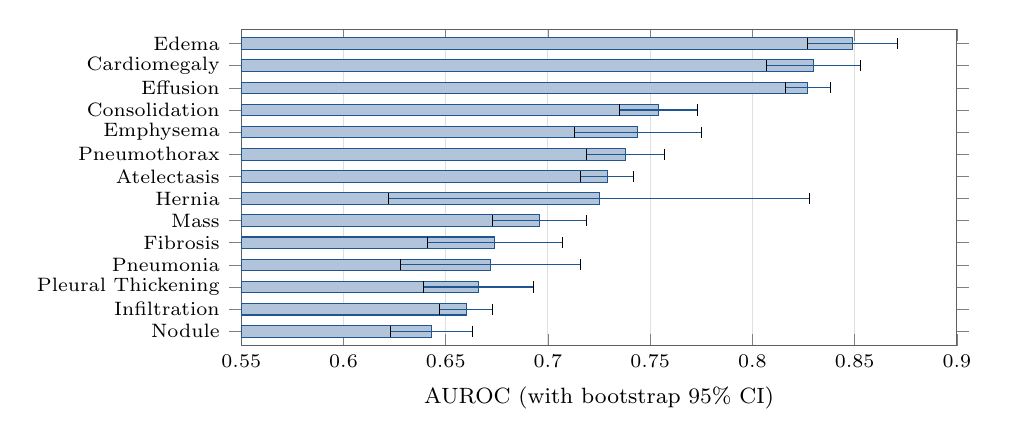
\begin{tikzpicture}
\begin{axis}[
  width=0.88\linewidth, height=5.6cm,
  xbar, xmin=0.55, xmax=0.90,
  bar width=4.2pt,
  enlarge y limits=0.05,
  symbolic y coords={Nodule,Infiltration,Pleural Thickening,Pneumonia,Fibrosis,
    Mass,Hernia,Atelectasis,Pneumothorax,Emphysema,Consolidation,Effusion,
    Cardiomegaly,Edema},
  ytick=data,
  xlabel={AUROC (with bootstrap 95\% CI)},
  xmajorgrids, grid style={gray!25},
  tick label style={font=\scriptsize},
  label style={font=\footnotesize},
  axis line style={mirrorgray},
]
\addplot[fill=mirrorblue!35, draw=mirrorblue, error bars/.cd,
         x dir=both, x explicit] coordinates {
  (0.643,Nodule)             +- (0.020,0)
  (0.660,Infiltration)       +- (0.013,0)
  (0.666,Pleural Thickening) +- (0.027,0)
  (0.672,Pneumonia)          +- (0.044,0)
  (0.674,Fibrosis)           +- (0.033,0)
  (0.696,Mass)               +- (0.023,0)
  (0.725,Hernia)             +- (0.103,0)
  (0.729,Atelectasis)        +- (0.013,0)
  (0.738,Pneumothorax)       +- (0.019,0)
  (0.744,Emphysema)          +- (0.031,0)
  (0.754,Consolidation)      +- (0.019,0)
  (0.827,Effusion)           +- (0.011,0)
  (0.830,Cardiomegaly)       +- (0.023,0)
  (0.849,Edema)              +- (0.022,0)
};
\end{axis}
\end{tikzpicture}
\caption{Per-label test AUROC on ChestMNIST (DenseNet-121, $64$\,px source upsampled
to $224$\,px, CPU, best of four epochs, $N_{\text{test}}{=}12{,}000$), with
bootstrap $95\%$ CI whiskers, sorted ascending. The ordering tracks how visible
each finding is, and every interval clears the $0.5$ chance line. Eleven of these
labels nonetheless emit no positive prediction at the default threshold
(Section~\ref{sec:operating}).}
\label{fig:cxr-auroc}
\end{figure}

\subsection{Harness control on synthetic data}
\label{sec:synthetic}
Numbers are only worth reporting if the harness that produced them credits real
signal and nothing else, so we test that directly. We train the same pipeline on a
fully synthetic dataset of $1{,}400$ procedurally generated chest-radiograph-like
images whose generator injects a visible blob for seven named labels, Mass, Nodule,
Effusion, Infiltration, Consolidation, Edema, and Cardiomegaly, and leaves the
other seven with no visual correlate. The seven are fixed in the generator in
advance, not chosen after seeing results.

A correct harness should learn exactly the first group and sit near chance on the
second, and that is what happens (Fig.~\ref{fig:synth}). On a $350$-image held-out
synthetic test split the seven signal-bearing labels reach a mean AUROC of $0.917$,
from Mass at $0.979$ down to Edema at $0.866$, and the seven no-signal labels
average $0.533$, from Hernia at $0.620$ down to Pleural Thickening at $0.434$. The
two groups do not overlap: the worst signal-bearing label outscores the best
no-signal label by $0.25$ AUROC. The no-signal mean sits slightly above $0.5$ and
straddles chance in both directions, which rules out a systematic leak. The
classifier, the loss, the metrics, and the bootstrap intervals therefore respond to
injected signal and not to label frequency or ordering.

\begin{figure}[tbp]
\centering
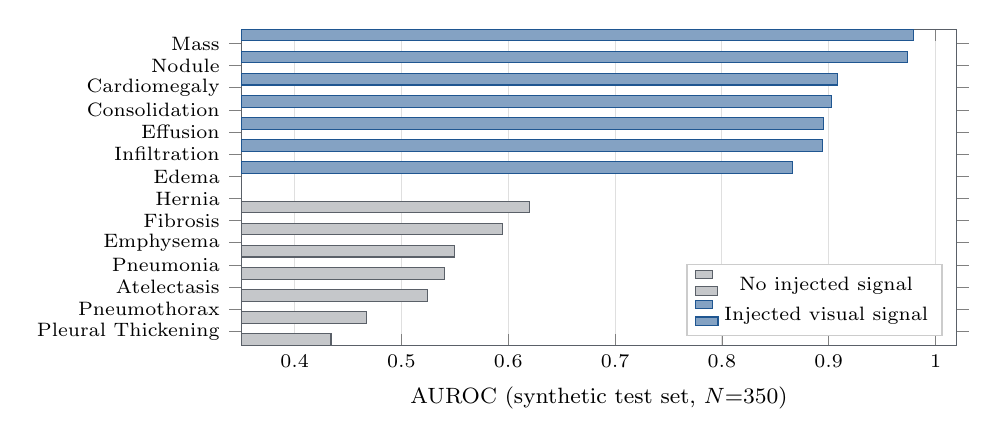
\begin{tikzpicture}
\begin{axis}[
  width=0.88\linewidth, height=5.6cm,
  xbar, xmin=0.35, xmax=1.02,
  bar width=4.2pt,
  enlarge y limits=0.05,
  symbolic y coords={Pleural Thickening,Pneumothorax,Atelectasis,Pneumonia,
    Emphysema,Fibrosis,Hernia,Edema,Infiltration,Effusion,Consolidation,
    Cardiomegaly,Nodule,Mass},
  ytick={Pleural Thickening,Pneumothorax,Atelectasis,Pneumonia,
    Emphysema,Fibrosis,Hernia,Edema,Infiltration,Effusion,Consolidation,
    Cardiomegaly,Nodule,Mass},
  xlabel={AUROC (synthetic test set, $N{=}350$)},
  xmajorgrids, grid style={gray!25},
  tick label style={font=\scriptsize},
  label style={font=\footnotesize},
  legend style={font=\scriptsize, at={(0.98,0.03)}, anchor=south east, draw=gray!40},
  axis line style={mirrorgray},
]
\addplot[fill=mirrorgray!35, draw=mirrorgray] coordinates {
  (0.434,Pleural Thickening) (0.467,Pneumothorax) (0.524,Atelectasis)
  (0.540,Pneumonia) (0.550,Emphysema) (0.595,Fibrosis) (0.620,Hernia)};
\addplot[fill=mirrorblue!55, draw=mirrorblue] coordinates {
  (0.866,Edema) (0.894,Infiltration) (0.895,Effusion) (0.903,Consolidation)
  (0.908,Cardiomegaly) (0.974,Nodule) (0.979,Mass)};
\legend{No injected signal, Injected visual signal}
\end{axis}
\end{tikzpicture}
\caption{Harness control on synthetic data. The generator injects a blob for seven
labels named in advance and none for the other seven; the classifier learns
\emph{exactly} the signal-bearing group (mean AUROC $0.917$) and stays near chance
on the rest (mean $0.533$), with no overlap. This checks that the metrics measure
real discrimination rather than label frequency, and that nothing is leaking.}
\label{fig:synth}
\end{figure}

\subsection{Post-hoc invariance and latency}
\label{sec:ablation}
Layers 2 and 3 run after the forward pass and modify no weights and no logits, so
the predictions are identical across the three conditions by construction. The
harness confirms it: the maximum per-label probability change against the
classification-only baseline is $0.000$ over $n{=}24$ studies. This is a regression
test, not a result. It earns its place because a nonzero delta would expose a real
bug, an accidental coupling between the layers, and the test suite asserts the same
property per modality against stubbed backbones so it holds structurally rather than
only for the chest checkpoint.

The cost that does vary is latency (Table~\ref{tab:ablation}). Prediction takes
about $100$\,ms per study on CPU, the Grad-CAM pass adds $36$ to $41$\,ms, and the
offline template report adds $0.03$\,ms. The two conditions that run Grad-CAM
measured $41.4$ and $36.2$\,ms for the same work, which is the run-to-run spread of
a 24-study CPU profile and is why the full-pipeline total of $136.2$\,ms came in
below the localization-only total of $140.9$\,ms. Interpretability here costs
roughly a $40\%$ increase in wall-clock time over a bare classifier: all of that
sits in the saliency pass, and none in the report.

\begin{table}[tbp]
\centering
\caption{Ablation conditions with measured per-stage wall-clock latency
(ms/study, mean over $24$ studies on CPU). Each row is a separate profiling run, so
its \emph{Predict} time carries the run-to-run spread of a 24-study CPU profile;
within each row \emph{Predict $+$ Localize $+$ Report} equals \emph{Total}. That
spread, not any change in work, is why full MIRROR totals less than localization
alone. \textbf{There is one AUROC measurement here, not three:} macro AUROC $=0.729$
from Table~\ref{tab:panel} applies unchanged to every row because the post-hoc
layers cannot alter a prediction.}
\label{tab:ablation}
\footnotesize
\begin{tabular}{@{}lrrrr@{}}
\toprule
\textbf{Condition} & \textbf{Predict} & \textbf{Localize} & \textbf{Report} & \textbf{Total} \\
\midrule
Classification only       & 101.2 & ---  & ---  & 101.2 \\
$+$ Evidence localization & \phantom{0}99.5 & 41.4 & ---  & 140.9 \\
Full MIRROR               & 100.0 & 36.2 & 0.03 & 136.2 \\
\midrule
\multicolumn{5}{@{}l}{\footnotesize Macro AUROC $=0.729$ in every row: one measurement.} \\
\multicolumn{5}{@{}l}{\footnotesize Max probability change vs.\ baseline $=0.000$, $n{=}24$.} \\
\bottomrule
\end{tabular}
\end{table}

% -----------------------------------------------------------------------------
\section{Multi-Modal Analysis by Construction}
\label{sec:multimodal}

Section~\ref{sec:method} introduced the registry in passing; here we make the
multi-modal claim explicit, because it is the transferable part of this work. The
argument is that a single analysis pipeline can span imaging modalities if, and only
if, the handful of things that actually differ between them are lifted out of the
code and into data.

\rih{What differs across modalities, and what does not.} Between a chest radiograph,
a brain MRI, and a head CT, three things change: the finding taxonomy the head
predicts (14 labels for chest X-ray, 11 each for brain MRI and head CT), the
anatomical vocabulary a saliency centroid is named in, and a little report phrasing,
so that a normal brain study reads ``no acute intracranial abnormality'' rather than
``no acute cardiopulmonary abnormality.'' Everything else, the backbone factory, the
multi-label head, the class-activation map, the $3\times3$ centroid-to-region
mapping, the evidence payload, and the report structure, is shared. MIRROR
centralizes exactly those three varying pieces in one registry
(Table~\ref{tab:modalities}), the single source of truth for each modality's labels,
glosses, imaging plane, and report guidance, so adding a fourth modality is a data
change and not a change to the pipeline.

\rih{Anatomical vocabulary follows the imaging plane.} The same $3\times3$ grid that
turns a saliency centroid into a named region is read through a per-modality plane.
For a frontal chest film the grid names lung zones; for an axial brain-MRI or
head-CT slice it names lobar regions, both in radiology convention with patient-right
on the viewer's left. The localizer computes one kind of map; the registry decides
what to call the place it points to. This is what lets a single localization layer
produce anatomically appropriate language for three modalities without any
modality-specific code.

\rih{Routing across modalities.} A study reaches the correct classifier head either
from an explicit selection or, for native DICOM, from the (0008,0060) modality tag
(MR to brain MRI, CT to head CT, CR or DX to chest X-ray). The DICOM ingest that
extracts that tag is the same one that applies the modality LUT, the VOI LUT, and
the MONOCHROME1 inversion, so heterogeneous real-world studies are both routed and
correctly rendered before the pipeline sees a pixel. The orchestrator builds and
caches one classifier-and-explainer engine per modality on demand, and a hand-kept
TypeScript mirror of the registry gives the hosted engine and the web interface the
identical taxonomy and \emph{ordering}, since output index $i$ maps to
$\text{labels}[i]$.

\rih{Cross-modal grounding: image to evidence to text.} MIRROR also crosses the
modality boundary between an image and its textual report, and this is where its one
non-obvious guarantee lives. The reasoning layer receives the structured evidence of
Fig.~\ref{fig:evidence}, labels, probabilities, and region names, and never the
pixels, so the language modality is a faithful re-expression of the image modality:
the report can assert only findings the classifier produced. Because both report
backends consume identical evidence, swapping them changes how fluently the report
reads, not which findings it asserts. That property is a consequence of the payload's
shape, so it is checkable by a unit test rather than a benchmark, and the same
post-hoc invariance is asserted per modality against stubbed backbones.

\rih{Scope, stated plainly.} The multi-modality claim is architectural and is scoped
as such. Routing, head sizing, anatomical vocabulary, and per-modality phrasing are
exercised by the test suite for all three taxonomies. No brain-MRI or head-CT
checkpoint has been trained, so MIRROR makes no predictive claim on those modalities;
what the registry demonstrates is that the pipeline is ready for them, not that it
has been evaluated on them. Everything measured in Section~\ref{sec:results} is chest
X-ray.

% -----------------------------------------------------------------------------
\section{Discussion}
\label{sec:discussion}

\rih{Finding-level grounding is a real guarantee and a narrow one.} Because the
language layer receives a label, a probability, and a region name rather than an
image (Fig.~\ref{fig:evidence}), the set of findings the report may assert is
exactly the set the classifier produced. That is checkable without trusting anything
about the model: a reader holding the report and the probability vector can verify
the correspondence, and a unit test can assert it. It is also strictly a claim about
\emph{which findings appear}, and says nothing about the sentences around them. A
report that correctly asserts consolidation may frame it with clauses the system
never computed, and those clauses inherit the credibility of the finding they sit
beside (Section~\ref{sec:ethics}). Architectures that constrain only the former
should say so rather than claiming groundedness in general.

\rih{Where this stands against Rudin.} MIRROR is precisely the architecture
Rudin~\cite{rudin2019stop} argues against for high-stakes decisions: an opaque CNN
with a saliency map and a language layer attached after the fact. We have no
rebuttal, and we do not claim the saliency map is faithful; the sanity checks of
Adebayo et al.~\cite{adebayo2018sanity} are the right instrument and we have not run
them. What we claim is narrower and does not depend on the heatmap being faithful:
the finding set is auditable, because a reader can check the report against the
probability vector directly. That is a retreat from explanation to auditability, and
we would rather name it than dress it up. An inherently interpretable classifier
would be the stronger answer.

\rih{Discrimination and decisions are different failures.} Macro AUROC $0.729$ reads
as a modest but working model. Brier $0.045$ and ECE $0.018$ read as a
well-calibrated one. AUPRC lift of $1.6$ to $6.8$ times prevalence says the ranking
is genuinely informative on every label. And the model emits no positive prediction
for 11 of 14 labels. All four statements are true simultaneously, which they can be
only because ranking quality and decision quality are separate properties that the
usual headline metrics do not distinguish. Reporting AUROC alone would have hidden
the failure; reporting the operating point alone would have hidden that the
representation is sound and the fix is a per-label threshold rather than a bigger
network. The practical recommendation is to publish sensitivity and PPV alongside
every AUROC in this literature, and to write both AUPRC and Brier against their
prevalence-derived floors.

\rih{One contract, two very different engines.} Serving the same JSON response from
a PyTorch stack and from a hosted vision LLM shows the \emph{interface} MIRROR
proposes, namely predict, show evidence, explain, is independent of the inference
backend, at the price of the asymmetry in Section~\ref{sec:serving}: the grounding
guarantee holds only on the local stack, and we flag that rather than let one
system's architecture diagram vouch for the other's behaviour.

% -----------------------------------------------------------------------------
\section{Ethics, Safety, and Limitations}
\label{sec:ethics}

\rih{Not a medical device.} MIRROR is a research prototype, not reviewed or cleared
by any regulatory body; every output is a draft that must be verified by a licensed
radiologist and must not be used for diagnosis or treatment. Each report carries
that disclaimer explicitly.

\rih{A worked example of ungrounded detail.} Fig.~\ref{fig:qual} shows a generated
report beside its evidence overlay. Two phrases in it are worth quoting: the cardiac
silhouette is described as normal \emph{with a cardiothoracic ratio below $0.5$},
and the \emph{costophrenic angles are noted to be clear}. The system measured
neither. No cardiothoracic ratio was computed, no cardiac or thoracic boundary was
segmented, and no costophrenic angle was localized; the pipeline produced a
probability per label and up to three saliency centroids, and nothing in that
evidence supports either clause. Both are fluent radiology register generated to
fill out a report. They also sit in the same paragraph as assertions that \emph{are}
grounded, and that adjacency is the danger: a reader who checks the consolidation
finding against the overlay and finds it correct has been given a reason to extend
trust to the sentence beside it. Fluency makes ungrounded detail more dangerous, not
less, because it arrives wearing the credibility of the verified finding next to it.
This is why finding-level grounding cannot be described as making a report safe, and
why the AI-generated-draft disclaimer is load-bearing rather than boilerplate.

\rih{Human subjects and data governance.} No ethics-board review was required: this
work uses only existing, public, de-identified benchmark datasets, namely NIH
ChestX-ray14 and its MedMNIST derivative, and collects no new data from human
subjects. Those datasets are governed by their own data use agreements; no raw
images, weights, or protected health information are committed to version control,
and the DICOM ingest extracts only non-PHI technical tags.

\rih{Limitations.} Our one quantitative benchmark is ChestMNIST, at $64$-pixel
source resolution on a $7{,}200$-image budget, and at its default threshold the
classifier is not a working detector (Section~\ref{sec:operating}). No clinical
claim of any kind follows from it. Multi-modality is architectural: the brain-MRI
and head-CT paths are implemented and exercised by the test suite but have no
trained checkpoints. Explanation quality is unmeasured: the pointing-game and IoU
protocol is implemented but not run, and no reader study has been conducted, so we
have no evidence that the localization or report layers help a human, only that they
cost about $40$\,ms. Report quality is assessed only qualitatively; a comparison
against real radiologist reports is future work.

% -----------------------------------------------------------------------------
\section{Conclusion}

MIRROR composes classification, evidence localization, and report generation into
one registry-driven pipeline that spans three imaging modalities by treating each
modality's taxonomy, anatomical vocabulary, and report phrasing as data rather than
code, and that crosses the image-to-text boundary under a grounding constraint
keeping the language layer faithful to the classifier's findings. Chest X-ray, brain
MRI, and head CT are registered, routed, and exercised by the test suite; adding a
fourth modality is a data change. We are deliberate about scope: only chest X-ray is
trained, and on the ChestMNIST derivative the classifier reaches macro AUROC $0.729$,
ranks every label between $1.6$ and $6.8$ times better than a random ranker, and
still emits no positive prediction for 11 of its 14 labels while posting a Brier
score within $0.002$ of a predictor that never looks at the image, a
decision-versus-discrimination gap we report against its no-skill floors. The
brain-MRI and head-CT paths are architectural. Next steps are training checkpoints
for those two modalities, full-resolution training on the NIH release, per-label
threshold selection on a validation split, the saliency sanity checks we cite but
did not run, and a reader study.

% -----------------------------------------------------------------------------
\section*{Reproducibility}
\footnotesize
Code: \url{https://github.com/vignesh-nagarajan-vn/MIRROR}. Live demo, on the hosted
engine: \url{https://mirror-ten-jet.vercel.app/}. A zero-setup CLI demo
(\code{python -m demo.run\_demo <image>}) runs the local pipeline on ImageNet weights
with the offline template backend, needing no checkpoint and no API key. Every
results JSON stamps a \code{reproducibility} block with the seed, git commit, and
library versions, and the unit tests are torch-free. The ChestMNIST result
(\code{configs/chestmnist.yaml}) and the synthetic control
(\code{configs/synthetic.yaml}) regenerate from seed $42$; their outputs are
committed under \code{results/}. The prevalences, the AUPRC lifts, the no-skill Brier
floor, and the exact contents of Table~\ref{tab:panel} are recomputed from those
files by \code{paper/calibration\_baseline.py}.

\section*{Acknowledgment}
This work was completed as part of the Global Indian Scientists \& Technocrats
(GIST) 2026 Summer Research Internship. The author thanks his mentor, Sriram
Venkatapathy, for guidance throughout the project.

% =============================================================================
\begin{thebibliography}{99}
\footnotesize
\setlength{\itemsep}{0pt}

\bibitem{wang2017chestxray}
X.~Wang, Y.~Peng, L.~Lu, Z.~Lu, M.~Bagheri, and R.~M. Summers,
``ChestX-ray8: Hospital-scale chest X-ray database and benchmarks on
weakly-supervised classification and localization of common thorax diseases,''
\emph{CVPR}, pp.~2097--2106, 2017.

\bibitem{rajpurkar2017chexnet}
P.~Rajpurkar, J.~Irvin, K.~Zhu, \emph{et al.},
``CheXNet: Radiologist-level pneumonia detection on chest X-rays with deep
learning,'' \emph{arXiv:1711.05225}, 2017.

\bibitem{irvin2019chexpert}
J.~Irvin, P.~Rajpurkar, M.~Ko, \emph{et al.},
``CheXpert: A large chest radiograph dataset with uncertainty labels and expert
comparison,'' \emph{AAAI}, 2019.

\bibitem{johnson2019mimiccxr}
A.~E.~W. Johnson, T.~J. Pollard, S.~J. Berkowitz, \emph{et al.},
``MIMIC-CXR, a de-identified publicly available database of chest radiographs with
free-text reports,'' \emph{Scientific Data}, vol.~6, no.~1, p.~317, 2019.

\bibitem{yang2023medmnist}
J.~Yang, R.~Shi, D.~Wei, Z.~Liu, L.~Zhao, B.~Ke, H.~Pfister, and B.~Ni,
``MedMNIST v2: A large-scale lightweight benchmark for 2D and 3D biomedical image
classification,'' \emph{Scientific Data}, vol.~10, no.~1, p.~41, 2023.

\bibitem{huang2017densenet}
G.~Huang, Z.~Liu, L.~van~der~Maaten, and K.~Q. Weinberger,
``Densely connected convolutional networks,'' \emph{CVPR}, pp.~4700--4708, 2017.

\bibitem{tan2019efficientnet}
M.~Tan and Q.~V. Le,
``EfficientNet: Rethinking model scaling for convolutional neural networks,''
\emph{ICML}, 2019.

\bibitem{dosovitskiy2021vit}
A.~Dosovitskiy, L.~Beyer, A.~Kolesnikov, \emph{et al.},
``An image is worth 16x16 words: Transformers for image recognition at scale,''
\emph{ICLR}, 2021.

\bibitem{zhou2016cam}
B.~Zhou, A.~Khosla, A.~Lapedriza, A.~Oliva, and A.~Torralba,
``Learning deep features for discriminative localization,'' \emph{CVPR},
pp.~2921--2929, 2016.

\bibitem{selvaraju2017gradcam}
R.~R. Selvaraju, M.~Cogswell, A.~Das, R.~Vedantam, D.~Parikh, and D.~Batra,
``Grad-CAM: Visual explanations from deep networks via gradient-based
localization,'' \emph{ICCV}, pp.~618--626, 2017.

\bibitem{wang2020scorecam}
H.~Wang, Z.~Wang, M.~Du, \emph{et al.},
``Score-CAM: Score-weighted visual explanations for convolutional neural
networks,'' \emph{CVPR Workshops}, 2020.

\bibitem{ribeiro2016lime}
M.~T. Ribeiro, S.~Singh, and C.~Guestrin,
``\,`Why should I trust you?': Explaining the predictions of any classifier,''
\emph{KDD}, pp.~1135--1144, 2016.

\bibitem{lundberg2017shap}
S.~M. Lundberg and S.-I. Lee,
``A unified approach to interpreting model predictions,'' \emph{NeurIPS}, 2017.

\bibitem{zhang2016pointing}
J.~Zhang, S.~A. Bargal, Z.~Lin, J.~Brandt, X.~Shen, and S.~Sclaroff,
``Top-down neural attention by excitation backprop,'' \emph{ECCV}, 2016.

\bibitem{adebayo2018sanity}
J.~Adebayo, J.~Gilmer, M.~Muelly, I.~Goodfellow, M.~Hardt, and B.~Kim,
``Sanity checks for saliency maps,'' \emph{NeurIPS}, 2018.

\bibitem{rudin2019stop}
C.~Rudin,
``Stop explaining black box machine learning models for high stakes decisions and
use interpretable models instead,'' \emph{Nature Machine Intelligence}, vol.~1,
no.~5, pp.~206--215, 2019.

\bibitem{doshivelez2017rigorous}
F.~Doshi-Velez and B.~Kim,
``Towards a rigorous science of interpretable machine learning,''
\emph{arXiv:1702.08608}, 2017.

\bibitem{wang2018tienet}
X.~Wang, Y.~Peng, L.~Lu, Z.~Lu, and R.~M. Summers,
``TieNet: Text-image embedding network for common thorax disease classification and
reporting in chest X-rays,'' \emph{CVPR}, 2018.

\bibitem{chen2020r2gen}
Z.~Chen, Y.~Song, T.-H. Chang, and X.~Wan,
``Generating radiology reports via memory-driven transformer,'' \emph{EMNLP}, 2020.

\bibitem{liu2019clinically}
G.~Liu, T.-M.~H. Hsu, M.~McDermott, \emph{et al.},
``Clinically accurate chest X-ray report generation,'' \emph{MLHC}, 2019.

\bibitem{tjoa2021survey}
E.~Tjoa and C.~Guan,
``A survey on explainable artificial intelligence (XAI): Toward medical XAI,''
\emph{IEEE TNNLS}, vol.~32, no.~11, pp.~4793--4813, 2021.

\bibitem{davis2006pr}
J.~Davis and M.~Goadrich,
``The relationship between precision-recall and ROC curves,'' \emph{ICML},
pp.~233--240, 2006.

\bibitem{saito2015prc}
T.~Saito and M.~Rehmsmeier,
``The precision-recall plot is more informative than the ROC plot when evaluating
binary classifiers on imbalanced datasets,'' \emph{PLOS ONE}, vol.~10, no.~3,
p.~e0118432, 2015.

\bibitem{guo2017calibration}
C.~Guo, G.~Pleiss, Y.~Sun, and K.~Q. Weinberger,
``On calibration of modern neural networks,'' \emph{ICML}, pp.~1321--1330, 2017.

\end{thebibliography}

\end{document}
